\let\negmedspace\undefined
\let\negthickspace\undefined
\documentclass[journal,12pt,twocolumn]{IEEEtran}
\usepackage{cite}
\usepackage{amsmath,amssymb,amsfonts,amsthm}
\usepackage{algorithmic}
\usepackage{graphicx}
\usepackage{textcomp}
\usepackage{xcolor}
\usepackage{txfonts}
\usepackage{listings}
\usepackage{enumitem}
\usepackage{mathtools}
\usepackage{gensymb}
\usepackage{comment}
\usepackage[breaklinks=true]{hyperref}
\usepackage{tkz-euclide} % loads  TikZ and tkz-base
\usepackage{listings}
\usepackage[latin1]{inputenc}                                
\usepackage{color}                                            
\usepackage{array}                                            
\usepackage{longtable}                                       
\usepackage{calc}                                             
\usepackage{multirow}                                         
\usepackage{hhline}                                           
\usepackage{ifthen}                                           
\usepackage{lscape}
\usepackage{caption}

\newtheorem{theorem}{Theorem}[section]
\newtheorem{problem}{Problem}
\newtheorem{proposition}{Proposition}[section]
\newtheorem{lemma}{Lemma}[section]
\newtheorem{corollary}[theorem]{Corollary}
\newtheorem{example}{Example}[section]
\newtheorem{definition}[problem]{Definition}
%\newtheorem{thm}{Theorem}[section] 
%\newtheorem{defn}[thm]{Definition}
%\newtheorem{algorithm}{Algorithm}[section]
%\newtheorem{cor}{Corollary}
\newcommand{\BEQA}{\begin{eqnarray}}
\newcommand{\EEQA}{\end{eqnarray}}
\newcommand{\define}{\stackrel{\triangle}{=}}
\theoremstyle{remark}
\newtheorem{rem}{Remark}
%\bibliographystyle{ieeetr}
\begin{document}
\providecommand{\pr}[1]{\ensuremath{\Pr\left(#1\right)}}
\providecommand{\prt}[2]{\ensuremath{p_{#1}^{\left(#2\right)} }}        % own macro for this question
\providecommand{\qfunc}[1]{\ensuremath{Q\left(#1\right)}}
\providecommand{\sbrak}[1]{\ensuremath{{}\left[#1\right]}}
\providecommand{\lsbrak}[1]{\ensuremath{{}\left[#1\right.}}
\providecommand{\rsbrak}[1]{\ensuremath{{}\left.#1\right]}}
\providecommand{\brak}[1]{\ensuremath{\left(#1\right)}}
\providecommand{\lbrak}[1]{\ensuremath{\left(#1\right.}}
\providecommand{\rbrak}[1]{\ensuremath{\left.#1\right)}}
\providecommand{\cbrak}[1]{\ensuremath{\left\{#1\right\}}}
\providecommand{\lcbrak}[1]{\ensuremath{\left\{#1\right.}}
\providecommand{\rcbrak}[1]{\ensuremath{\left.#1\right\}}}
\newcommand{\sgn}{\mathop{\mathrm{sgn}}}
\providecommand{\abs}[1]{\left\vert#1\right\vert}
\providecommand{\res}[1]{\Res\displaylimits_{#1}} 
\providecommand{\norm}[1]{\left\lVert#1\right\rVert}
%\providecommand{\norm}[1]{\lVert#1\rVert}
\providecommand{\mtx}[1]{\mathbf{#1}}
\providecommand{\mean}[1]{E\left[ #1 \right]}
\providecommand{\cond}[2]{#1\middle|#2}
\providecommand{\fourier}{\overset{\mathcal{F}}{ \rightleftharpoons}}
\newenvironment{amatrix}[1]{%
  \left(\begin{array}{@{}*{#1}{c}|c@{}}
}{%
 \end{array}\right)
}
%\providecommand{\hilbert}{\overset{\mathcal{H}}{ \rightleftharpoons}}
%\providecommand{\system}{\overset{\mathcal{H}}{ \longleftrightarrow}}
        %\newcommand{\solution}[2]{\textbf{Solution:}{#1}}
\newcommand{\solution}{\noindent \textbf{Solution: }}
\newcommand{\cosec}{\,\text{cosec}\,}
\providecommand{\dec}[2]{\ensuremath{\overset{#1}{\underset{#2}{\gtrless}}}}
\newcommand{\myvec}[1]{\ensuremath{\begin{pmatrix}#1\end{pmatrix}}}
\newcommand{\mydet}[1]{\ensuremath{\begin{vmatrix}#1\end{vmatrix}}}
\newcommand{\myaugvec}[2]{\ensuremath{\begin{amatrix}{#1}#2\end{amatrix}}}
\providecommand{\rank}{\text{rank}}
\providecommand{\pr}[1]{\ensuremath{\Pr\left(#1\right)}}
\providecommand{\qfunc}[1]{\ensuremath{Q\left(#1\right)}}
        \newcommand*{\permcomb}[4][0mu]{{{}^{#3}\mkern#1#2_{#4}}}
\newcommand*{\perm}[1][-3mu]{\permcomb[#1]{P}}
\newcommand*{\comb}[1][-1mu]{\permcomb[#1]{C}}
\providecommand{\qfunc}[1]{\ensuremath{Q\left(#1\right)}}
\providecommand{\gauss}[2]{\mathcal{N}\ensuremath{\left(#1,#2\right)}}
\providecommand{\diff}[2]{\ensuremath{\frac{d{#1}}{d{#2}}}}
\providecommand{\myceil}[1]{\left \lceil #1 \right \rceil }
\newcommand\figref{Fig.~\ref}
\newcommand\tabref{Table~\ref}
\newcommand{\sinc}{\,\text{sinc}\,}
\newcommand{\rect}{\,\text{rect}\,}
%%
%       %\newcommand{\solution}[2]{\textbf{Solution:}{#1}}
%\newcommand{\solution}{\noindent \textbf{Solution: }}
%\newcommand{\cosec}{\,\text{cosec}\,}
%\numberwithin{equation}{section}
%\numberwithin{equation}{subsection}
%\numberwithin{problem}{section}
%\numberwithin{definition}{section}
%\makeatletter
%\@addtoreset{figure}{problem}
%\makeatother

%\let\StandardTheFigure\thefigure
\let\vec\mathbf

\bibliographystyle{IEEEtran}

\vspace{3cm}
\title{Assignment}
\author{EE23BTECH11008 - Meenakshi}
\maketitle
\newpage
\bigskip

\renewcommand{\thefigure}{\theenumi}
\renewcommand{\thetable}{\theenumi}
%\renewcommand{\theequation}{\theenumi}
Q:The difference between any two cosecutive interior angles of a polygon is $5^\circ$.If the smallest angle is $120^\circ$,find the number of sides of polygon.
\\\solution
The interior angles of a polygon are in AP with
    $x(0)=120$, $d=5$
\begin{table}[ht]
  \centering
  \begin{tabular}{|c|c|c|}
    \hline
      \textbf{Variable}& \textbf{Description}& \textbf{Value}\\\hline
    $x(0)$& first term of AP& 120  \\\hline
    d& common difference of AP & 5\\\hline
    $x(n)$ & general  term of AP&none\\\hline
   n & Describing the order of term & none\\\hline
    $u(n)$& unit step function & mentioned above\\\hline
    $U(z) $& z-transform of u(n) & $\frac{1}{1-z^{-1}}$\\\hline
    $X(z)$& z-transform of x(n) & $x(0)U(z)+d\left(-z\frac{d(U(z))}{dz}\right)$\\ 
    \hline
  \end{tabular}
  \end {table}
The sum of n terms of an AP is given by
\begin{equation}
    S=\frac{n}{2}(2\cdot x(0)+(n-1)d)
\end{equation}
Sum of interior angles of AP is given by
\begin{equation}
    S=(n-2)180
\end{equation}
\begin{align}
\frac{n}{2}(2\cdot x(0)+(n-1)d)&= (n-2)180\\
    \frac{n}{2}(240+(n-1)5)&=(n-2)180\\
    n(235+5n)&=360n-720\\
    5n^2+235n&=360n-720\\
    5n^2-125+720&=0\\
    n^2-25n+144&=0
\end{align}
solving the above equation we get
\begin{align}
   n=16,9
\end{align}
\begin{align}
 \boxed{x(n)=(120-5n)\times u(n)}   
\end{align}
\begin{figure}[h]
  \centering
  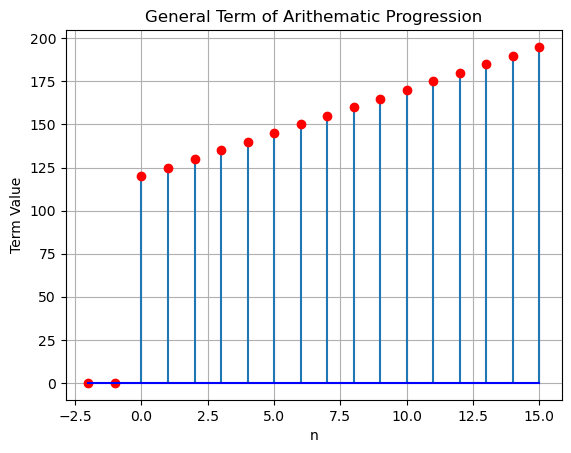
\includegraphics[width=0.5\linewidth]{/home/meena/figs/python.1(1).png} 
  \captionsetup{justification=centering}
  \caption{Plot of the general term taken from Python}
  \label{fig:your_label}
\end{figure}
The expression for u(n) is 
\[ u(n) = \begin{cases}
    1 & \text{if } n \geq 0, \\
    0 & \text{if } n < 0.
\end{cases} \]
On Z-transformation
\[\begin{aligned}
U(z)&=\sum\limits_{n=-\infty}^{\infty}z^{-n}u(n)\\
U(z)&=\sum\limits_{n=0}^{\infty}z^{-n}\\
\frac{d(U(z))}{dz}&=\sum\limits_{n=0}^{\infty}-nz^{-n-1}\\
\end{aligned}\]
Now,
\[\begin{aligned}
   X(z)&=\sum\limits_{n=-\infty}^{\infty}(x(0)+nd)z^{-n}u(n)\\
   X(z)&=x(0)U(z)+d\left(-z\frac{d(U(z))}{dz}\right)\\
   X(z)&=120U(z)+5\left(-z\frac{d(U(z))}{dz}\right)\\
   X(z)&=\frac{120}{1-z^{-1}}+\frac{5z^{-1}}{(1-z^{-1})^2}\hspace{5pt}
   \text{ROC: $|z|>1$}
\end{aligned}\]

\begin{align}
 \boxed{X(z)=120U(z)-5z\frac{d(U(z))}{dz}}  
\end{align}

\end{document}
   


